
\subsection*{task 1.5 \\[1ex] getting used to slicing (part 2)}

Read image \texttt{portrait.png} into an array \texttt{arrF}. Then ---without using \keyword{for} loops--- set all the intensities of the pixels in in every $16$th column and every $16$th row of \texttt{arrF} to $0$. Write your result as a PNG image.

To illustrate how this image should look like, here is the result you would obtain from working with every $8$th row and column and setting intensities to $255$.
%%%%%
%%%%%
%%%%% enter your result here, i.e. replace "t1-5.png" by the name of your resulting image file
%%%%%
%%%%%
\begin{center}
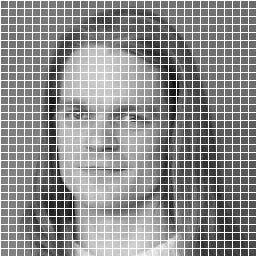
\includegraphics[width=0.5\textwidth]{t1-5.png} 
\end{center}
%%%%%
%%%%%
%%%%%
%%%%%
%%%%%
Simply replace the above image with the image you just created.






